\documentclass[11pt,a4paper]{article}

\usepackage[utf8x]{inputenc}   % omogoča uporabo slovenskih črk kodiranih v formatu UTF-8
\usepackage[slovene]{babel}    % naloži, med drugim, slovenske delilne vzorce

\usepackage[hyphens]{url}
\usepackage{hyperref}

\usepackage{graphicx}


\title{Akcijski načrt za mojo diplomsko nalogo:\\
Uporaba in analiza Monte-Carlo drevesnega preiskovanja na strateški igri}
\author{Jernej Habjan\\
jh0228@student.uni-lj.si\\
\ \\
predvideni MENTOR: doc. dr. Matej Guid \\
Fakulteta za računalništvo in informatiko Univerze v Ljubljani
\date{\today}         
}



\begin{document}
\maketitle

\section{Potrebne aktivnosti za izdelavo moje diplomske naloge}
\begin{itemize}
\item izdelava strateške igre,
\item raziskava algoritma,
\item implementacija algoritmov,
\item ovrednotenje rezultatov,
\item pisanje diplomske naloge,
\item zagovor.
\end{itemize}

\subsection{Izdelava strateške igre}
Igro moram izdelati v celostnem pogonu Unreal Engine 4.
Igra bo realno-časovna, kar pomeni, da jo moram dobro optimizirati, če hočem poganjati hevristične preiskovalne algoritme. V tem okolju bom lažje zasnoval grafično prezentacijo algoritma.
\begin{itemize}
	\item izdelava poganjalca algoritma,
	\item izdelava osebkov,
	\item predelava stanja igre.
\end{itemize}
Izdelati moram poganjalca algoritma, ki bo izbral določen algoritem in z njim igral proti nasprotniku.
Prav tako moram izdelati osebke in njihove akcije (npr. postavi hišo).
Te osebke bom pa hranil v stanju igre, ki pa ga algoritem uporablja, ki je abstrakcija za to, kateri osebki in akcije so trenutno na voljo.


\subsection{Raziskava algoritmov}
Ko bom imel izdelano ogrodje strateške igre, se bom lahko posvetil algoritmom.
Preiskal bom algoritme:
\begin{itemize}
\item Monte-Carlo drevesno preiskovanje,
\item variacija Monte-Carla, in sicer Naiven MCTS,
\item metode ocenjevanja CAB, UCB1,
\end{itemize}
Prav tako bom moral hkrati opisati, zakaj sem se za kateri algoritem odločil.

\subsection{Implementacija algoritma}
Ko bom imel algoritem dokončan, ga bom lahko implementiral v igro.
Postopek implementacije bo naslednji:
\begin{itemize}
\item implementacija Min-Max algoritma,
\item implementacija naključnega MCTS,
\item sprememba MCTS, da uporablja pravilne ocene,
\item sprememba preiskovalnega parametra pri ocenjevanju.
\end{itemize}

\subsection{Ovrednotenje rezultatov}
Ovrednotenje rezultatov bo pa potekalo po naslednjih korakih:
\begin{itemize}
\item simulacija igre računalnika proti računalniku (več sto simulacij),
\item igranje računalnika proti človeku (testiranje znancev).
\end{itemize}
Pri simulaciji računalnika proti računalniku, se bom osredotočil na rezultate kot so naprimer povprečno število simulacij pri MCTS algoritmu in konsistentnost ukazov.
Pri igranju proti človeku bom pa analiziral nekaj odločitvenih dreves ki jih je računalnik zgeneriral in ocenil odločitve na podlagi mojega predznanja igre.

\subsection{Pisanje diplomske naloge}
Pisanje diplomske naloge bo potekalo med raziskovanjem algoritmov in ovrednotenjem rezultatom.
Prav tako bom opisal zakaj sem izbral določen algoritem in kaj mi doprinese k rezultatu.
Opisal bom tudi celostni pogon Unreal Engine 4 in kratek opis strateške igre Trump Defense 2020.
\subsection{Zagovor}
Za zagovor moram pripraviti prosojnice v Microsoft Office, ki bodo glavna podlaga pri prezentaciji.
Prav tako bom moral pripraviti video, v katerem bom lahko predstavil igro in končen rezultat.

\section{Kako so identificirane aktivnosti povezane med seboj}

Na sliki \ref{sl:mreza} je mrežni diagram za izdelavo moje diplomske naloge.

\begin{figure}[htb]
\centerline{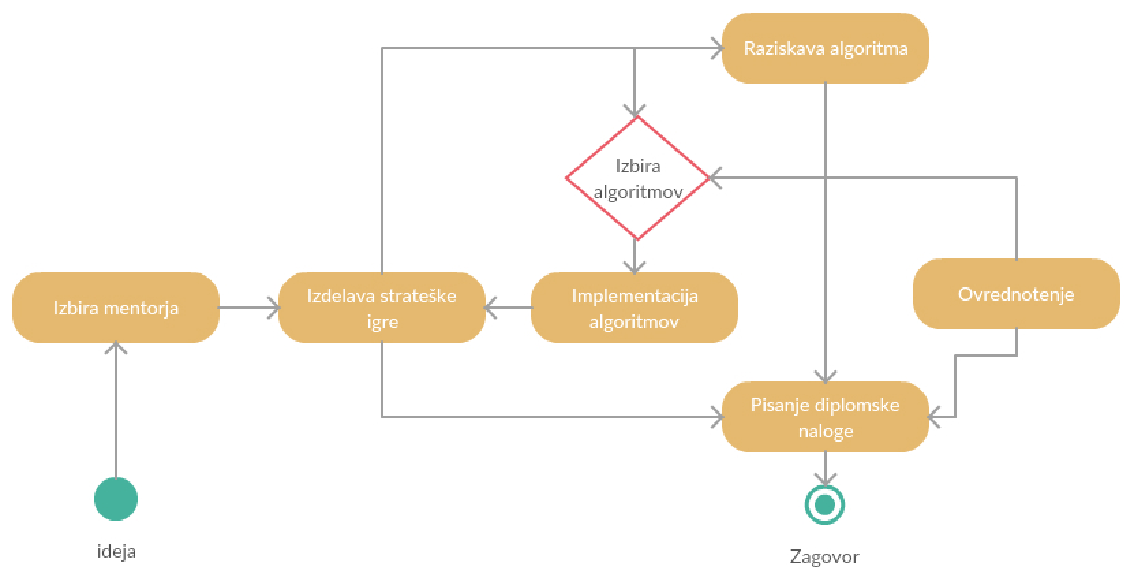
\includegraphics[width=1.0\textwidth]{DiplomskaNalogaDiagramPoteka.pdf}}
\caption{Mrežni diagram aktivnosti za mojo diplomsko nalogo.}
\label{sl:mreza}
\end{figure}

Na sliki je razvidno, da se bom večkrat vračal k izbiri algoritmov, saj jih bom moral vedno dopolnjevati, ker bodo slabo ovrednoteni.
Prav tako bom sproti moral pisati diplomsko nalogo in med razvijanjem algoritma vedno posodabljati igro.

\section{Časovna analiza in optimizacija načrta}

Čas izdelave strateške igre bo med študijem trajal še kakšen mesec, je pa igra v izdelavi že dva meseca. Raziskava algoritmov bo hitrejša operacija, saj je potencialni mentor doc. Matej Guid v preteklosti že veliko delal s takimi algoritmi, in me bo hitro znal usmeriti.
Ta proces zna trajati kakšen teden, saj bom sproti dopolnjeval diplomsko nalogo.
Ko bom našel primerne algoritme, jih bom moral implementirati, kar pomeni, da bom moral predelati igro in hkrati testirati če algoritem dela. To lahko traja 2 meseca med študijem.
Potem bom moral še ovrednotiti rezultate, kar lahko traja tudi kakšen mesec, ker bom ugotovil, da algoritem ne dela dovolj dobro in ga bom spreminjal.
Diplomsko nalogo bom pa pisal en mesec.

Skupen čas celotnega projekta potem znaša približno 6 mesecev prekinjajočega dela.
Imam še štiri mesece dela za diplomsko nalogo, kar je spremenljiv čas, glede na to, da je še prvi semester.

Kritična aktivnost je implementacija algoritma, saj moram še dobro raziskati kako bi se lotil rešitve in vpeljati različne vrste algoritmov v realno-strateško igro.


\section{Akcijski načrt}
Prvo moram narediti ogrodje igre v Unreal Engine 4. Ko bo to narejeno, bom lahko začel razvijati algoritem in začel pisati diplomsko nalogo.


\end{document}  




